
\cleardoublepage


\chapter{Northeast Beam Port Modeling}


% ------------------------------------------------------------------------------
\section{Tally Results}

Write about the tallying in general.

Write about the tallying in general.

Write about the tallying in general.

Write about the tallying in general.

Write about the tallying in general.

Write about the tallying in general.

% this image depicts the nebp flux as a function of energy
\begin{figure}[htb]
\centering
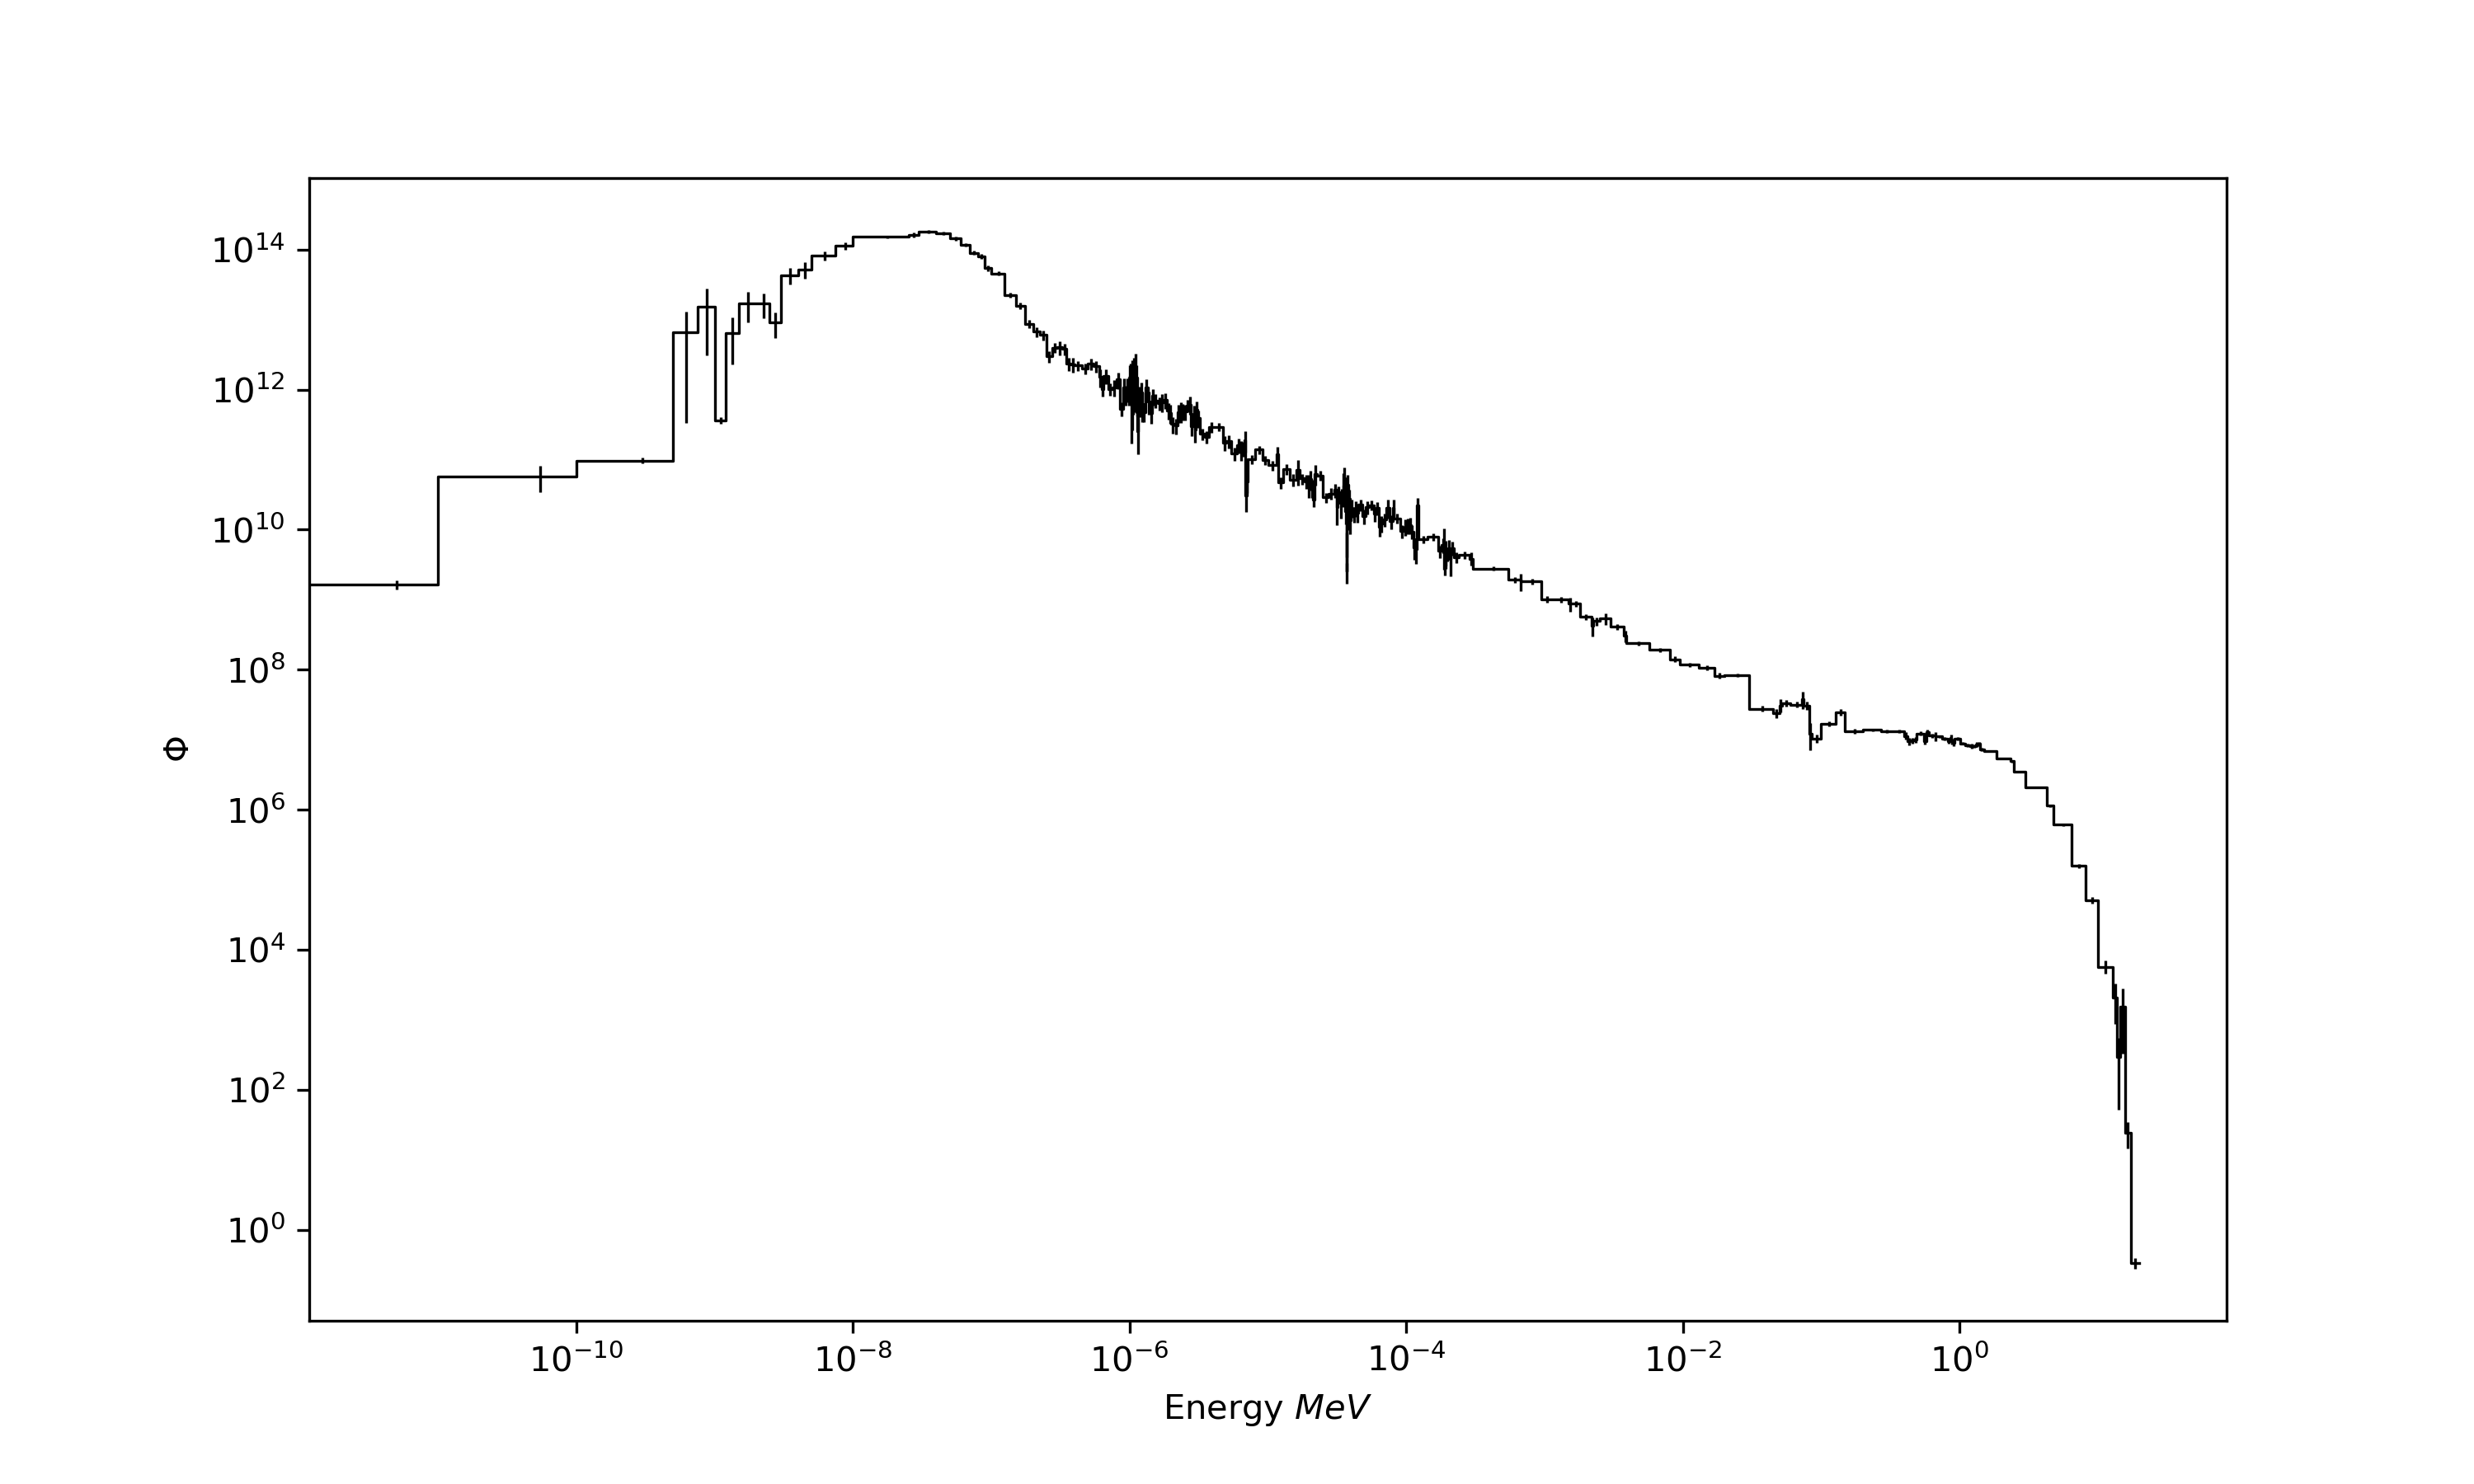
\includegraphics[height=4in]{tex/figures/flux_erg.png}
\caption[Flux vs. Energy]{The differential flux as a function of energy.}
\label{fig:flux_erg}
\end{figure}

% this is the differential flux as a function of energy
Shown in \FIG{fig:flux_erg} is the differential flux as a function of energy.
% it has been integrated over both angle and tally region
This has been integrated over both angle as well as the seven tally regions.
% because of this, the spectrum resembles that which one would find within the core
The spectrum resembles that which one would find within a reactor core.
% you've got your watt distribution % you've got your 1/E region % you've got your maxwellian distrubution
Centered around 1 MeV is the Watt fission distribution, the intermediate region is comprised of $1/E$ slowing down neutrons, and peaking around $3 \times 10^{-8}$ is the Maxwellian distribution.
% the main contribution to this tally is line of sight down the beam
This is likely because the line-of-sight neutrons streaming from the core are the primary component to this flux tally.
% as you can see, those are clearly on display because, ya know it should look like that
The borated polyethylene within the collimator is a very strong absorber and also very long, so it's unlikely that moderated neutrons escape and manage to contribute to the tally.

% there are two noisy locations
There are also two regions seen in this plot that are heavily affected by statistical noise, the slower half of the $1/E$ region and the slow tail of the Maxwellian distribution.
% this is because of low probability tallies
This is because there is such a low probability that a neutron at that energy will be tallied.
% this is because of small bin widths in the 1/e region and low probability within the super slow region
Specifically, within the scale252 bin structure, there are several narrow bins within the $1/E$ region, and tally probability is proportional to the bin width times the true flux, therefore, it's reasonable to see high errors within that region.
The flux in the tail end of the Maxwellian distribution is also very low, causing the poor resolution within that region.
These could ultimately be resolved via simulation of more particles.


\clearpage

%
\begin{figure}[htb]
\centering
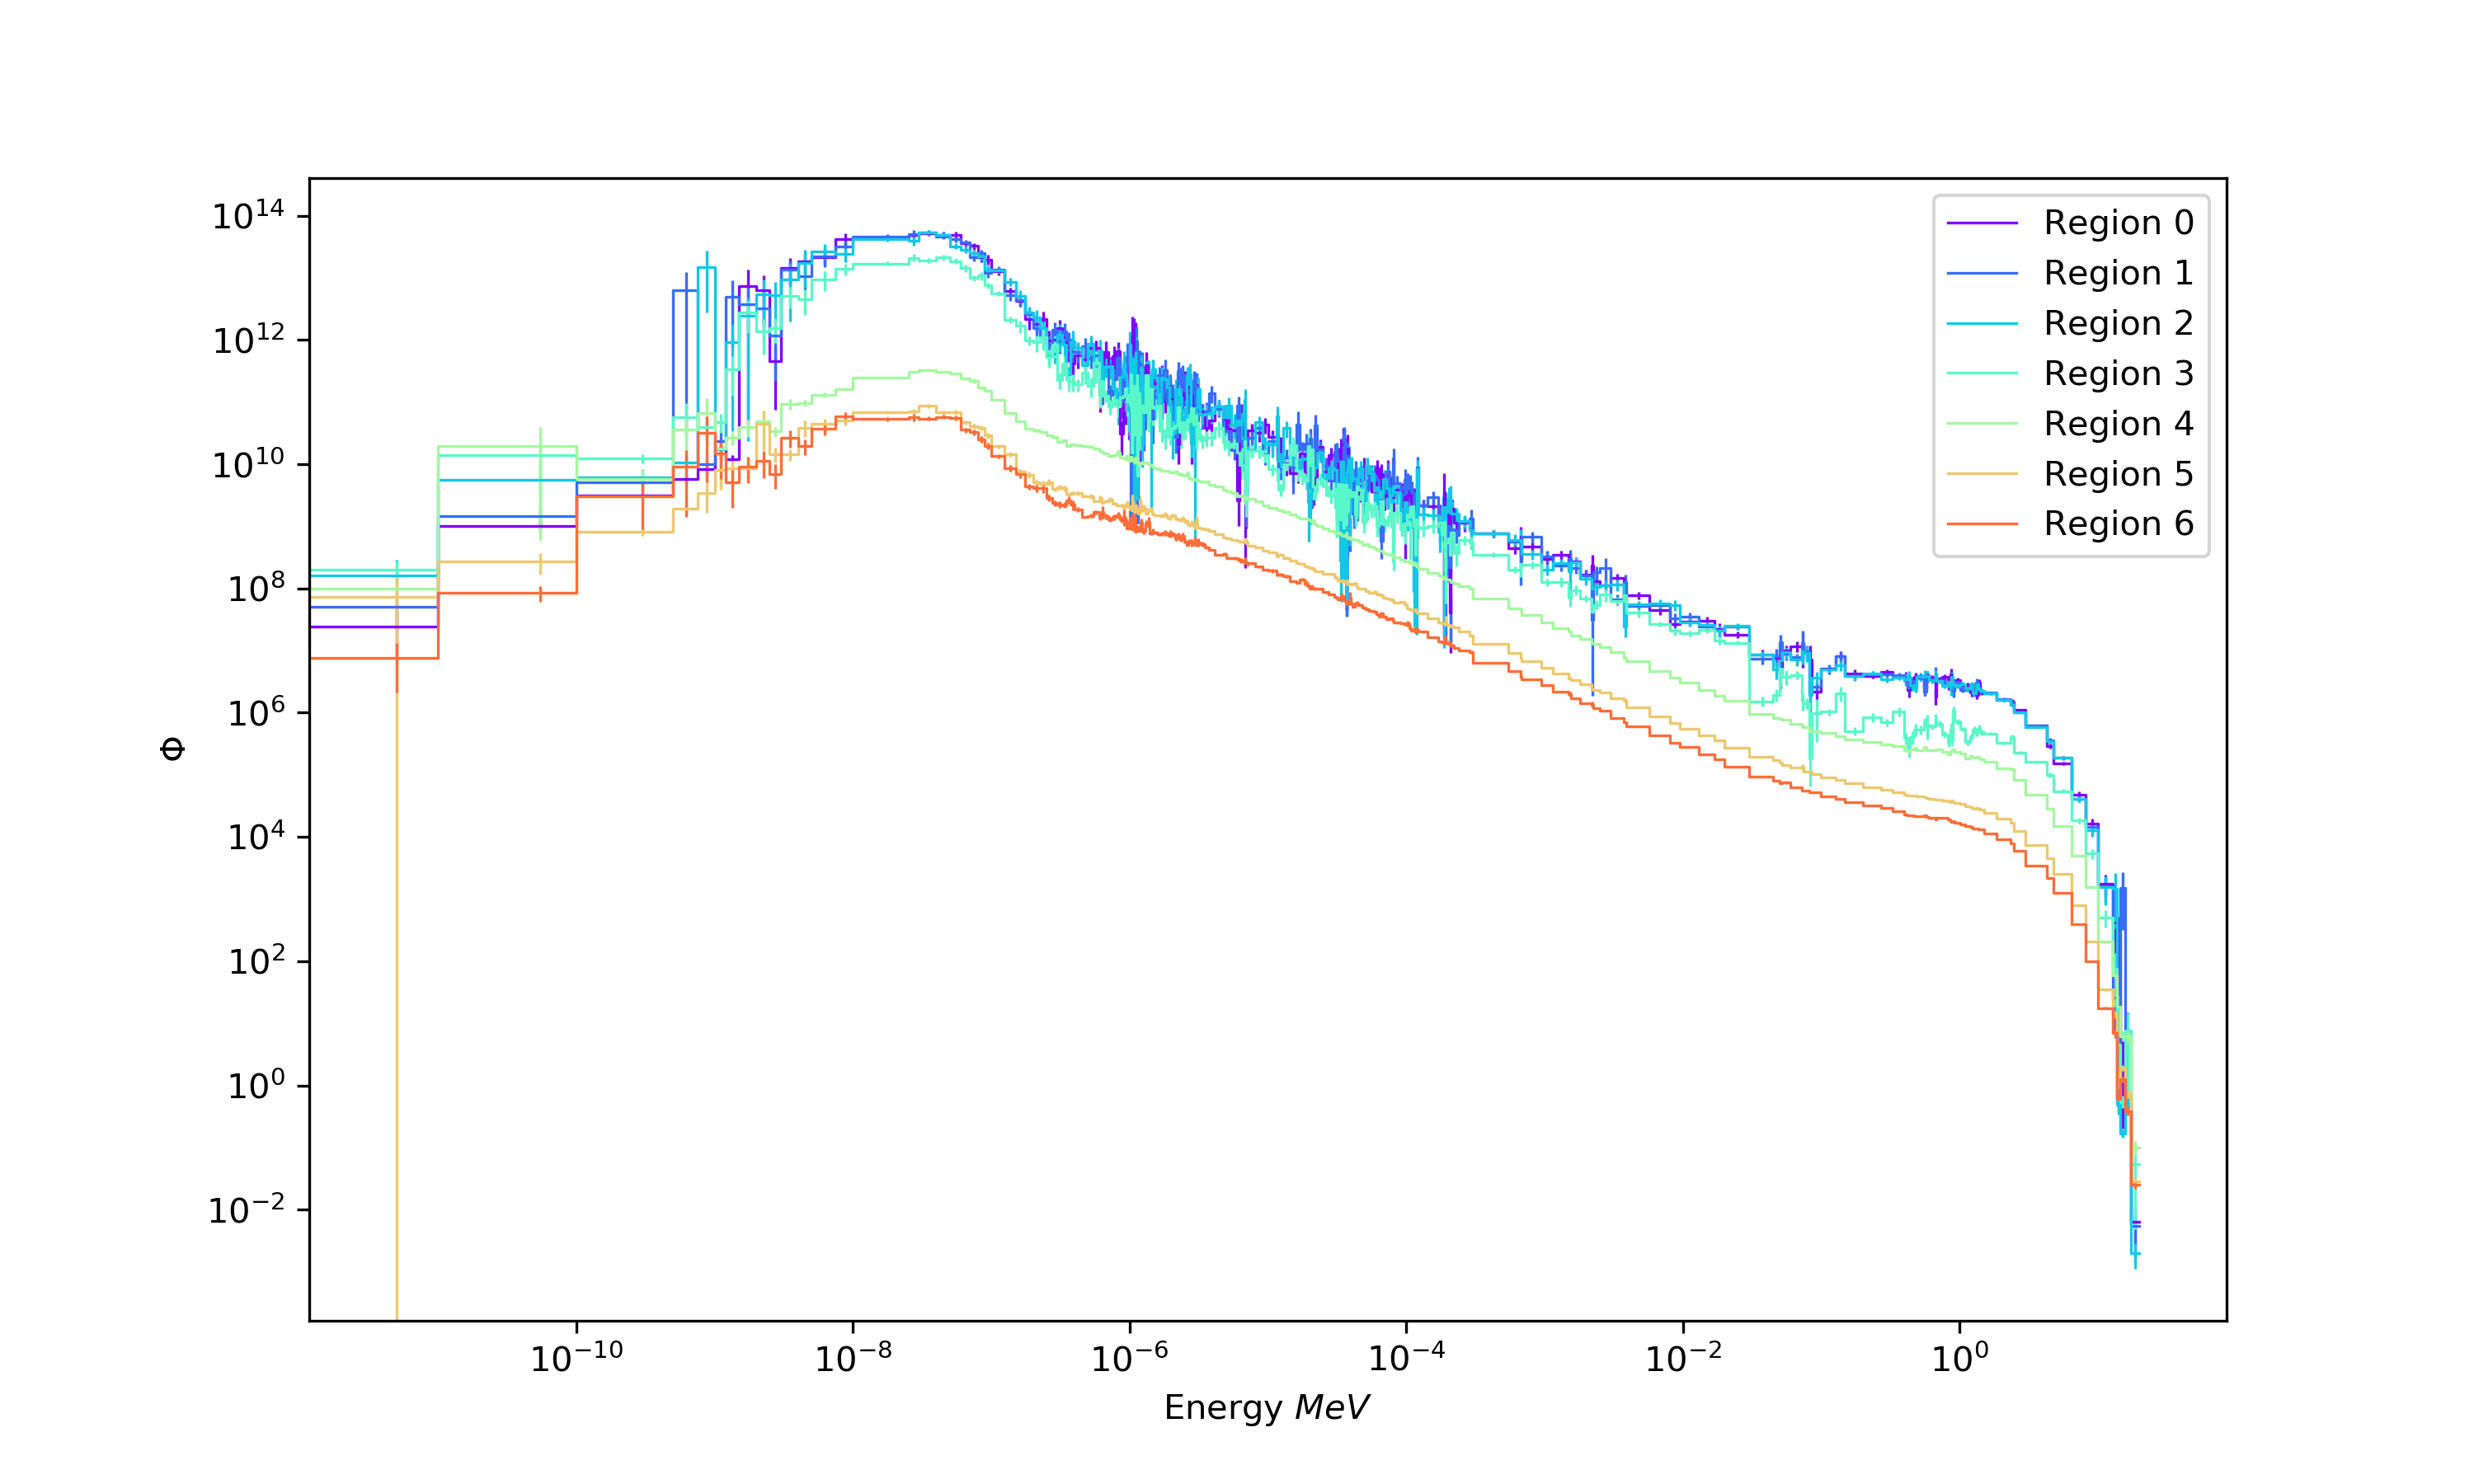
\includegraphics[height=4in]{tex/figures/flux_rad_erg.png}
\caption[Regional Flux vs. Energy]{The differential flux plotted against energy and broken into each tally region.}
\label{fig:flux_rad_erg}
\end{figure}

% the erg dependent flux can be seen broken down into region in figure whatever.
The energy-dependent flux can be seen broken down into it's separate regional tallies within \FIG{fig:flux_rad_erg}.
% regions 0-7 refer to whatever
Recall, regions 0-2 are equal-area tallies within the beam, region 3 refers to the aluminum collimator, and regions 5-7 are equal-area tallies within the borated polyethylene.
% this gives us a first glance at comparing magnitudes
This plot gives us a first glance at comparing the magnitudes within each region.
Over three orders of magnitude lie between the highest and lowest regional fluxes here.
% let's comment on noise for a sec, too
The noise problem \FIG{fig:flux_erg} is also amplified here, as separating the tallies by region furthur slows individual tally bin convergence.
However, it's still possible to draw meaningful conclusions from this plot.
% okay, first, there's like no difference in the first three
First, apart from statistical noise, there's no obvious difference between the spectra within the in-beam regions.
% in the aluminum, the fast flux seems flattened
It's in the aluminum where the flux begins to depart, being separated both by magnitude and also exibiting a flatness within the fast region.
% the bp sections are clearly moderated
Differences seen in the borated polyethylene regions are much more obvious, as the spectra are clearly moderated variants of those in-beam.
% look how the fast peak shrinks the further out you go
The furthur from the center of the beam, the more flat the fast region becomes.
% the 1/e region shows some curvature here. interesting
The $1/E$ region begins to demonstrate some curvature, which is likely in relation to the absorption and scattering cross sections of the borated polyethylene.
% also, maxwell is flattened
The Maxwellian distributions within these sections are also flattened and exibit much less drastic tapering in the slowest regions.

\clearpage

%
\begin{figure}[htb]
\centering
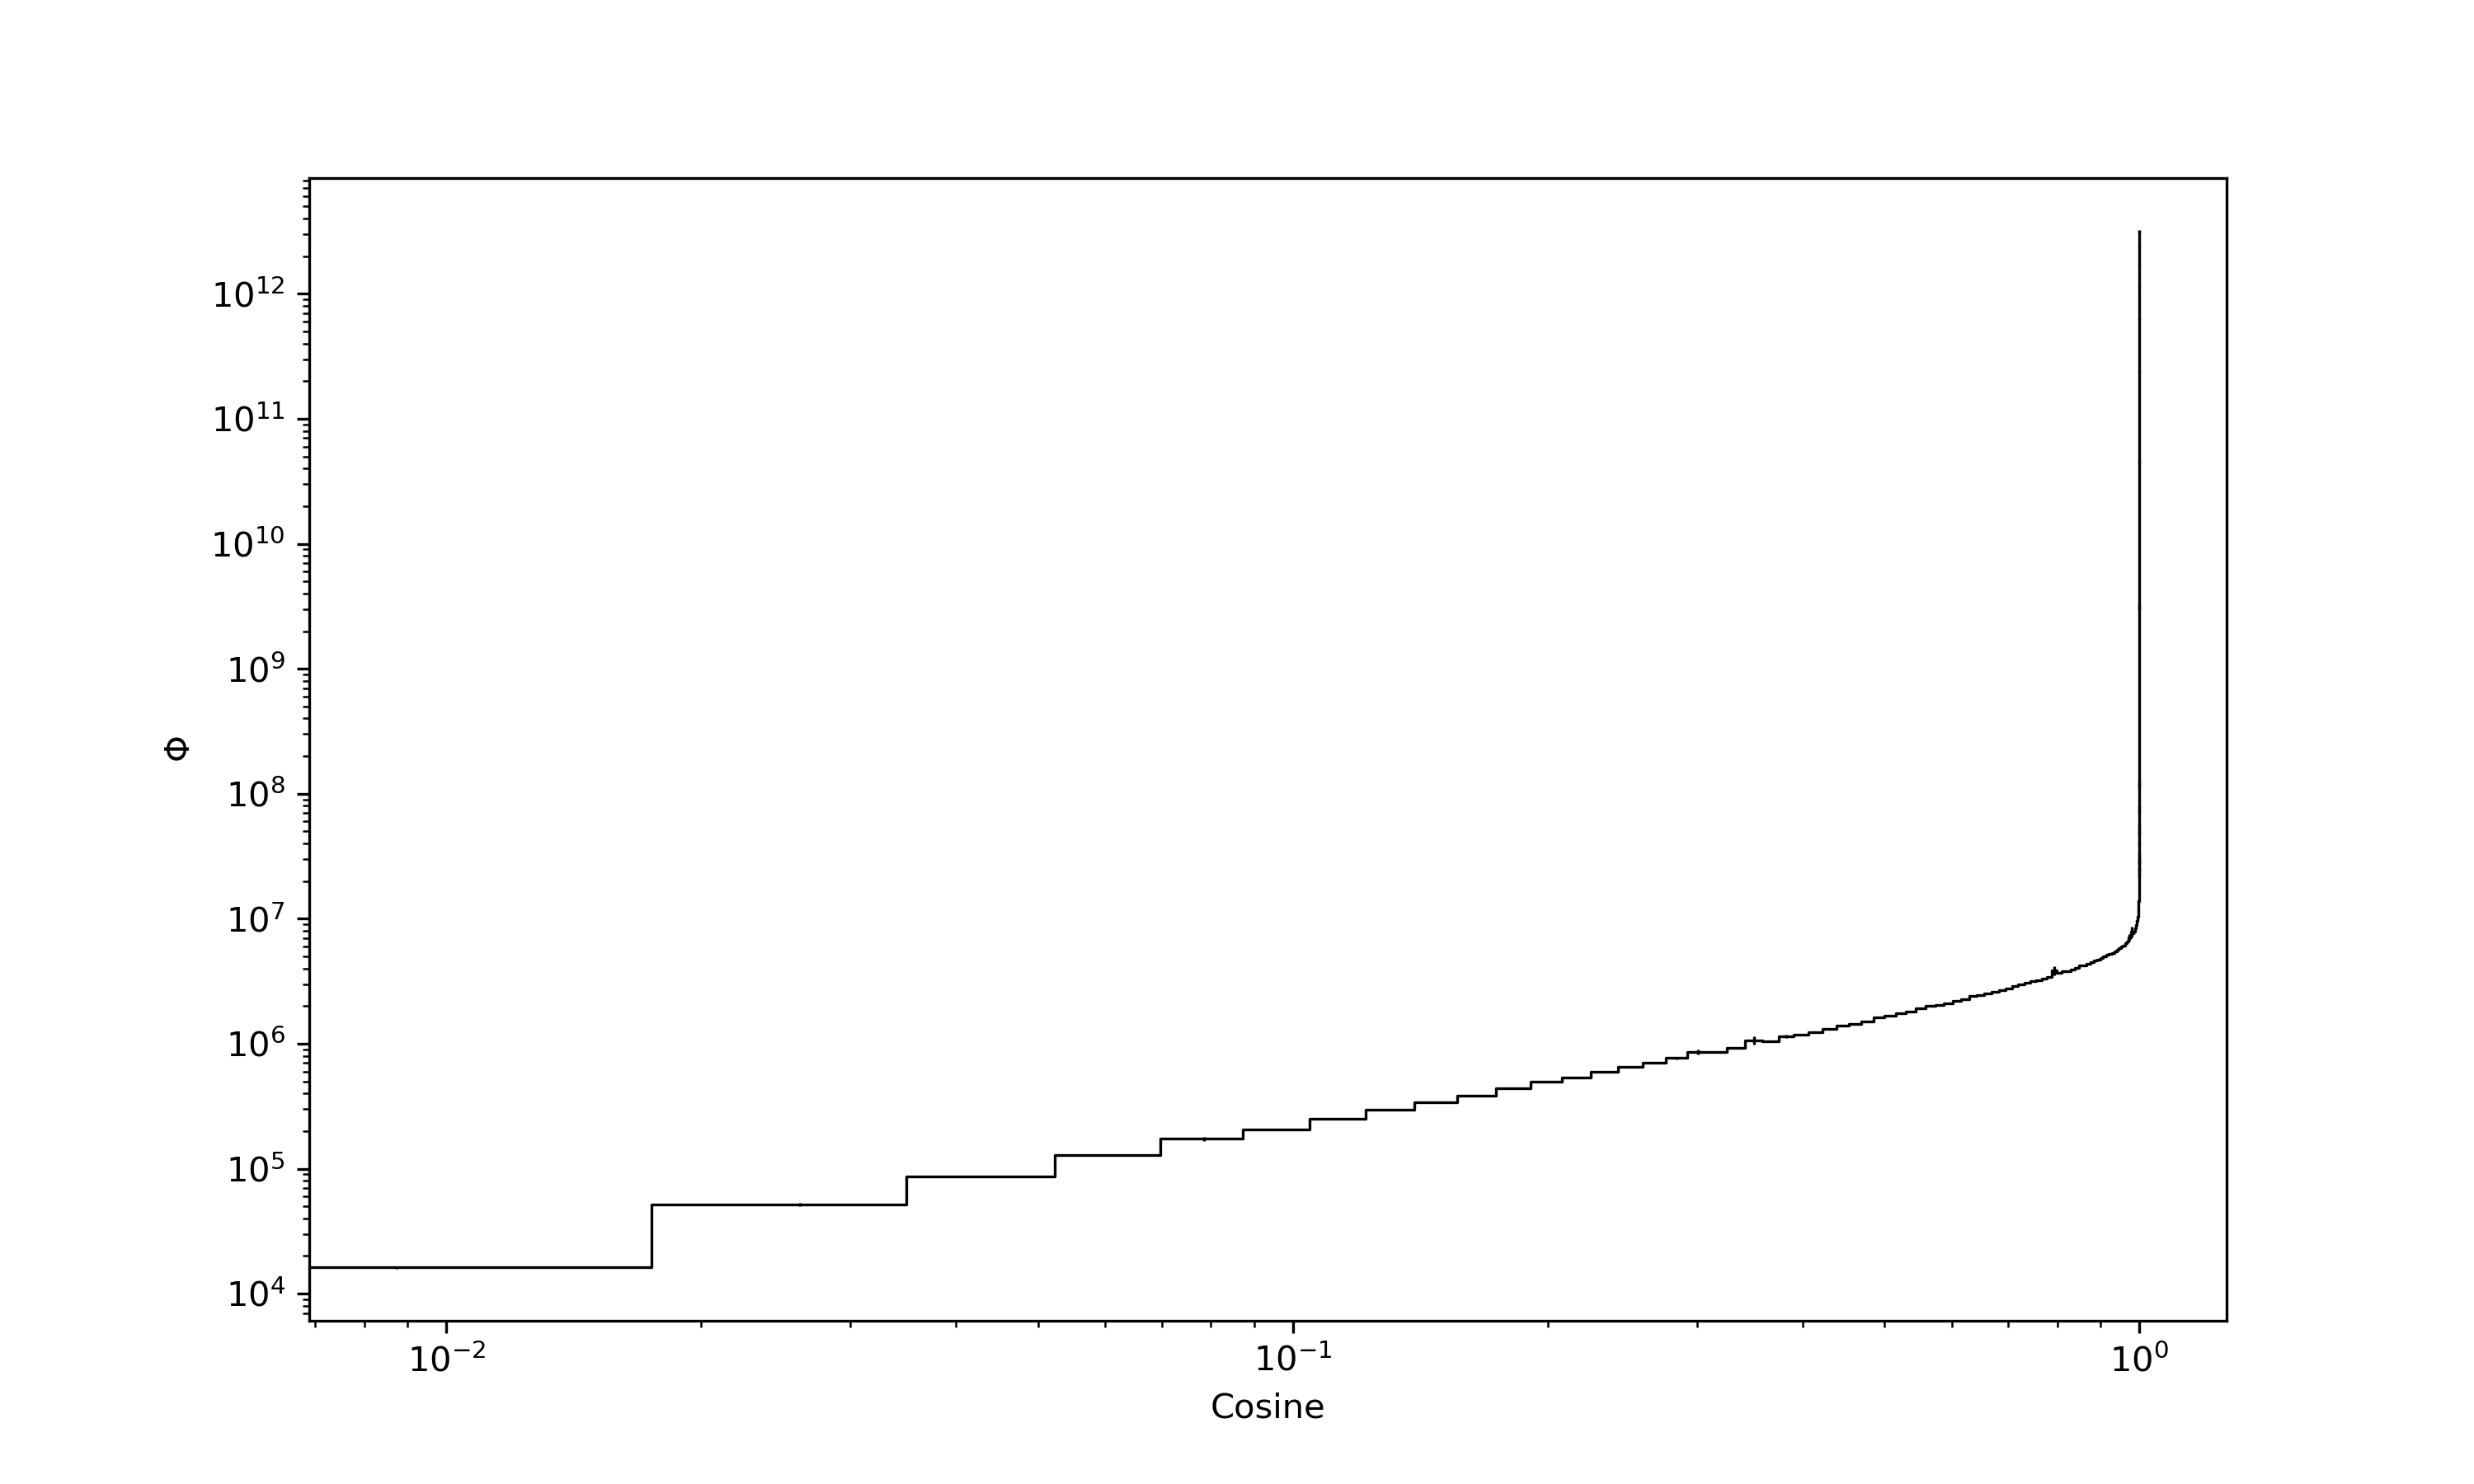
\includegraphics[height=4in]{tex/figures/flux_cos.png}
\caption[Flux vs. Angle]{The differential flux as a fuction of angle.}
\label{fig:flux_cos}
\end{figure}

% this is the figure showing the flux as a function of angle from
The flux as a function of angle can be seen in \FIG{fig:flux_cos}.
% right away, it's apparent that the collimator is doing its job
Right away, it is apparent that the collimator is effectively constricting the neutron beam.
% these fluxes span N orders of magnitude across the way
The fluxes in the plot span over eight orders of magnitude.
% the sharp increase at the right is caused by the line-of-sight through the beam
This incredibly sharp upturn at the right is due to the line-of-sight neutrons again being the largest contributor to the flux.
% outside of that, there's just a gradual exponential decrease as you go off beam through the BP region
Outside of that, the rest of this flux is goverened by a smooth exponential tapering caused by scattering within the collimator.

\clearpage

%
\begin{figure}[htb]
\centering
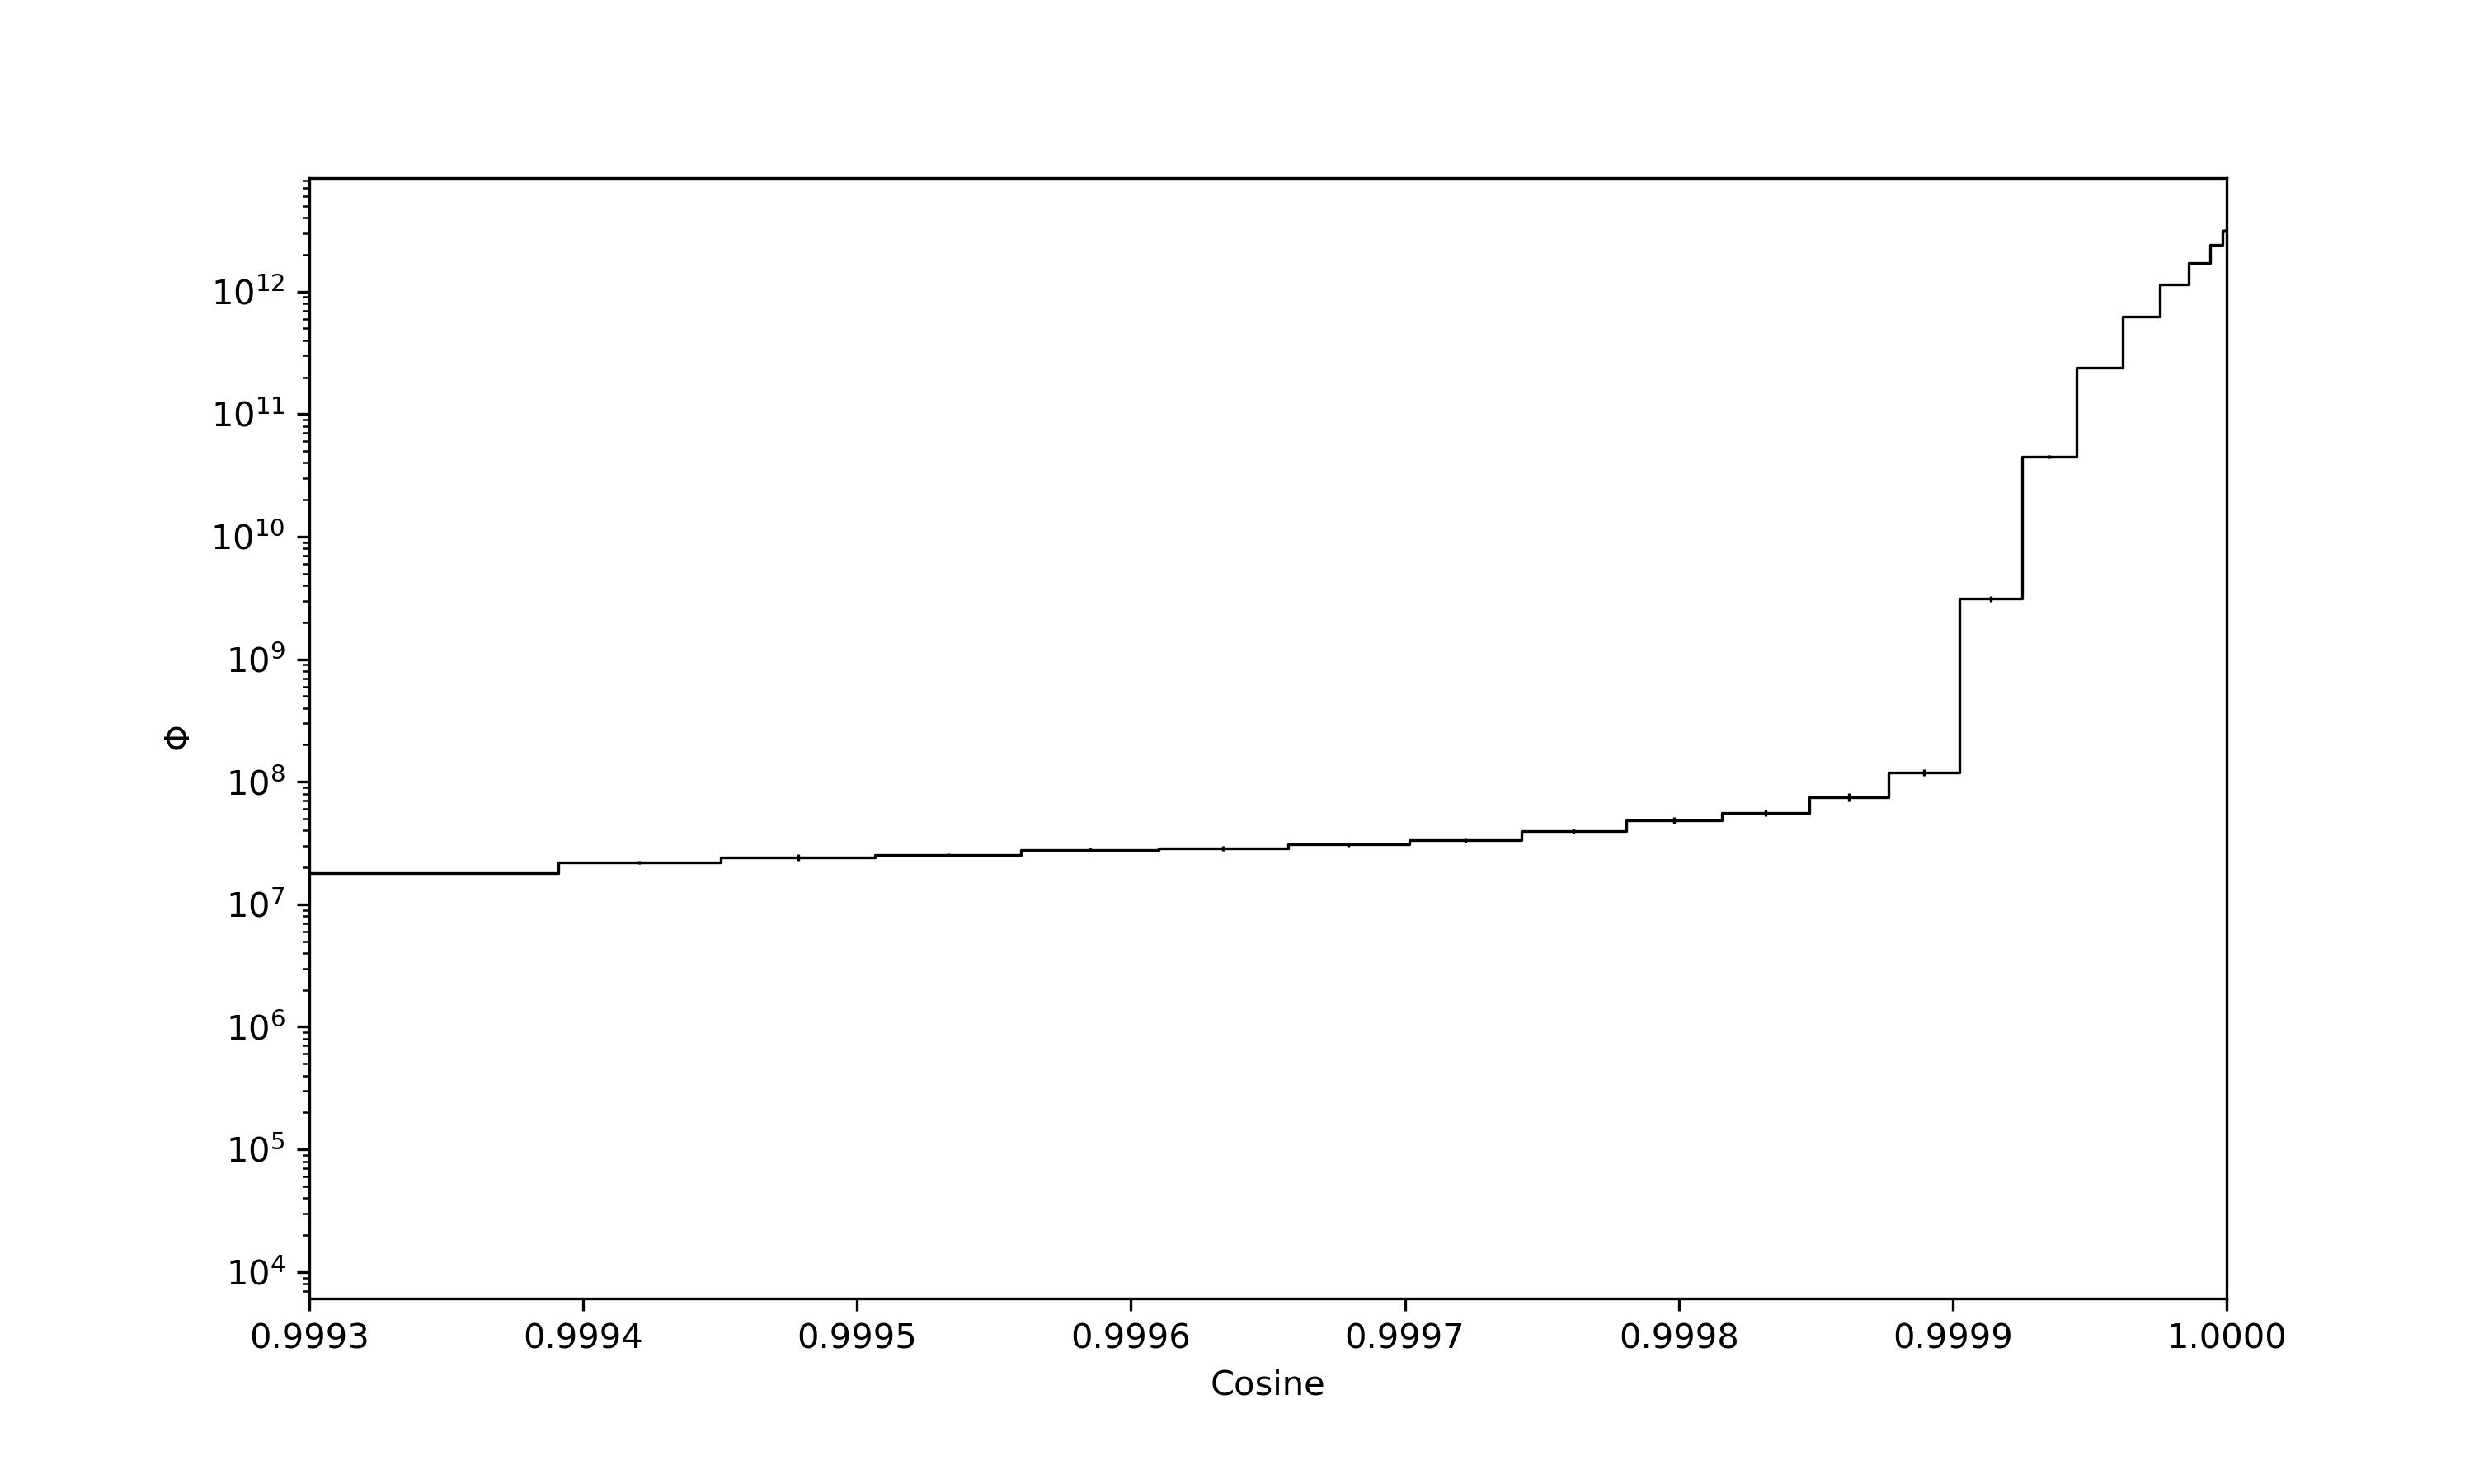
\includegraphics[height=4in]{tex/figures/flux_cos_detail.png}
\caption[Detailed Flux vs. Angle]{A detailed view of the NEBP angular flux.}
\label{fig:flux_cos_detail}
\end{figure}

% this is a closer look a the peak angular flux
Seen in \FIG{fig:flux_cos_detail} is a closer look at the forward peak in the angular flux.
% within a cosine of 0.9999 and 1.0000 there's a jump of over 5 orders of magnitude.
Within cosine values of 0.9999 and 1.0000 there's a jump of over five orders of magnitude.
% this allows us to comment on the relationship between scattering and absorption within the collimator
This allows us to comment on the relationship between scattering and absorption within the collimator.
% bounds on the sharpness of the peak matches the maximum angle that a neutron can travel within the collimator without an interaction.
The bounds on the sharpness of the peak match the maximum line-of-sight angle within the aluminum tube in the beam.
The neutrons within this peak are managing to stream down the collimator from the core without interacting on the way.
% if scattering was dominant within the collimator, this peak would appear much flatter, but since it's not, the boron within the collimator is likely the reason.
This suggests that it's absorption, not scattering that dominates interactions with in the collimator.
If scattering was more likely, this peak would be much smoother, but instead the neutrons entering the collimator are being removed.

\clearpage

% the radial flux broken into tally regions
\begin{figure}[htb]
\centering
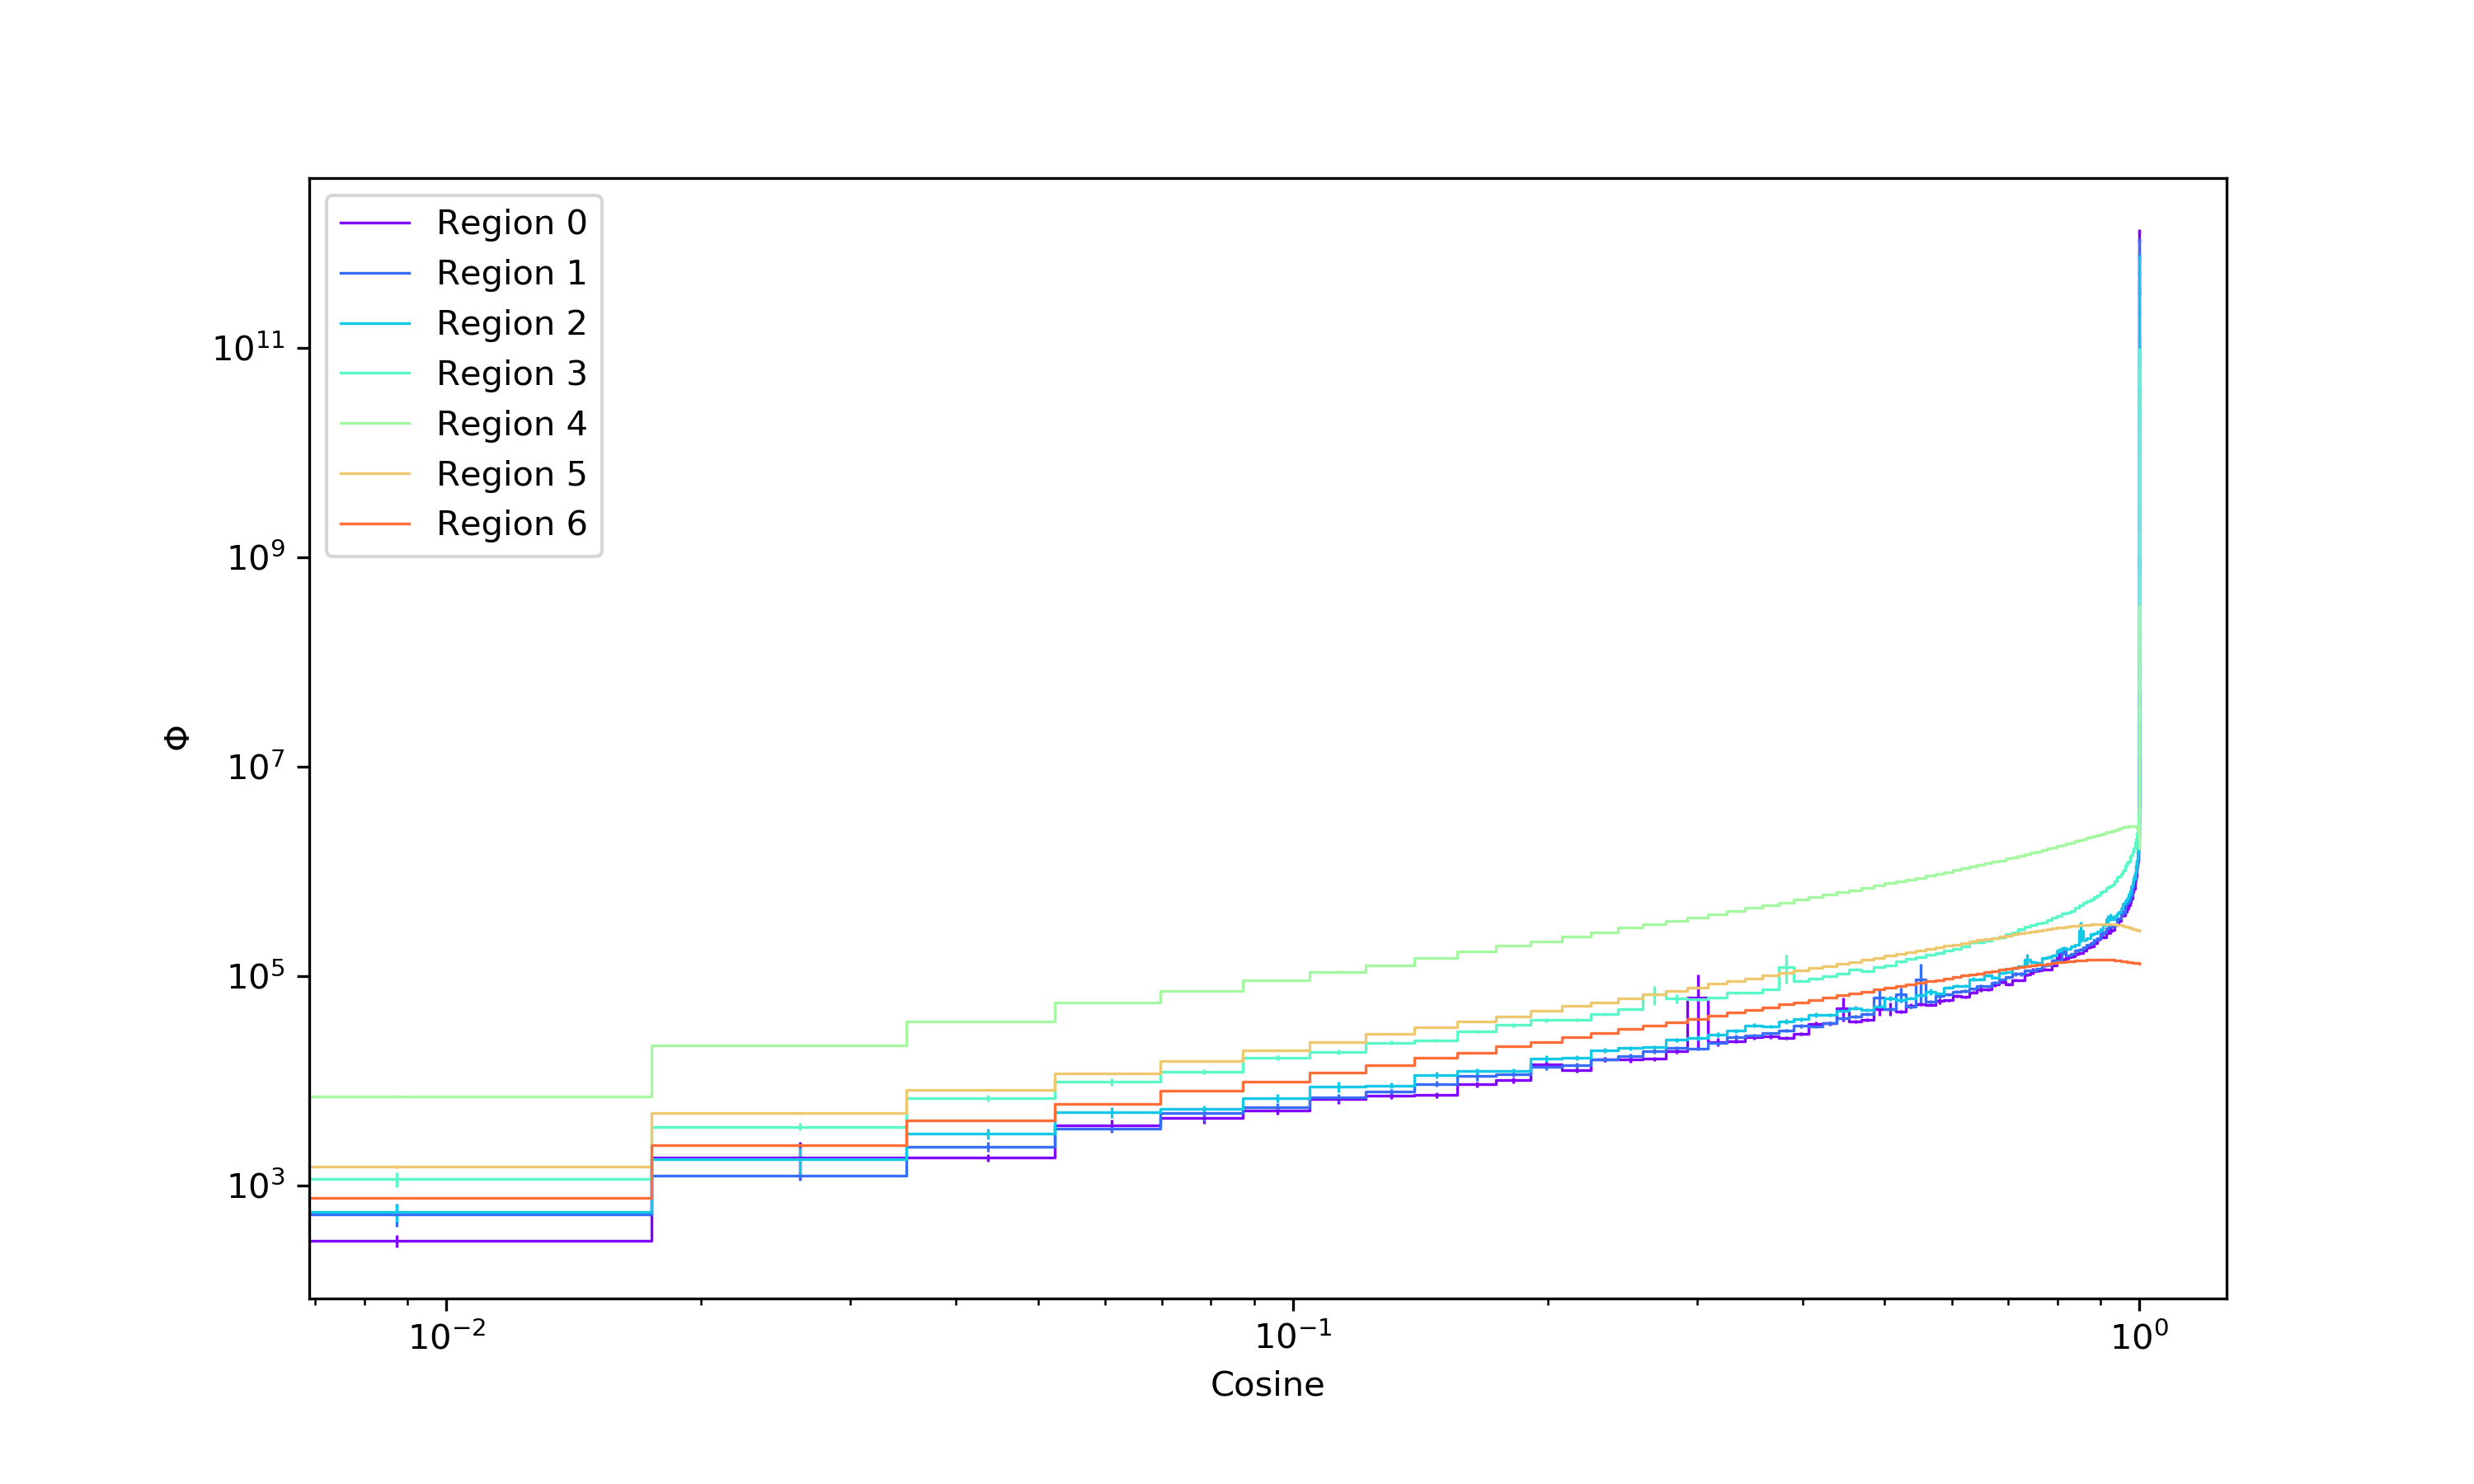
\includegraphics[height=4in]{tex/figures/flux_rad_cos.png}
\caption[Regional Flux vs. Angle]{The NEBP radial flux broken into tally regions.}
\label{fig:flux_rad_cos}
\end{figure}

% regional angular flux shown here
% similar to energy dependent flux, there's little deviation that can be seen between regions 0-2, except there's question about the magnitude here
% definite jump in the aluminum section
% the anisotropy is much higher within the outer regions
% they are still forward peaked, though, but that doesn't happen cos=1.000 but rather at an angle.

\clearpage

% detailed view of the regional flux vs angle
\begin{figure}[htb]
\centering
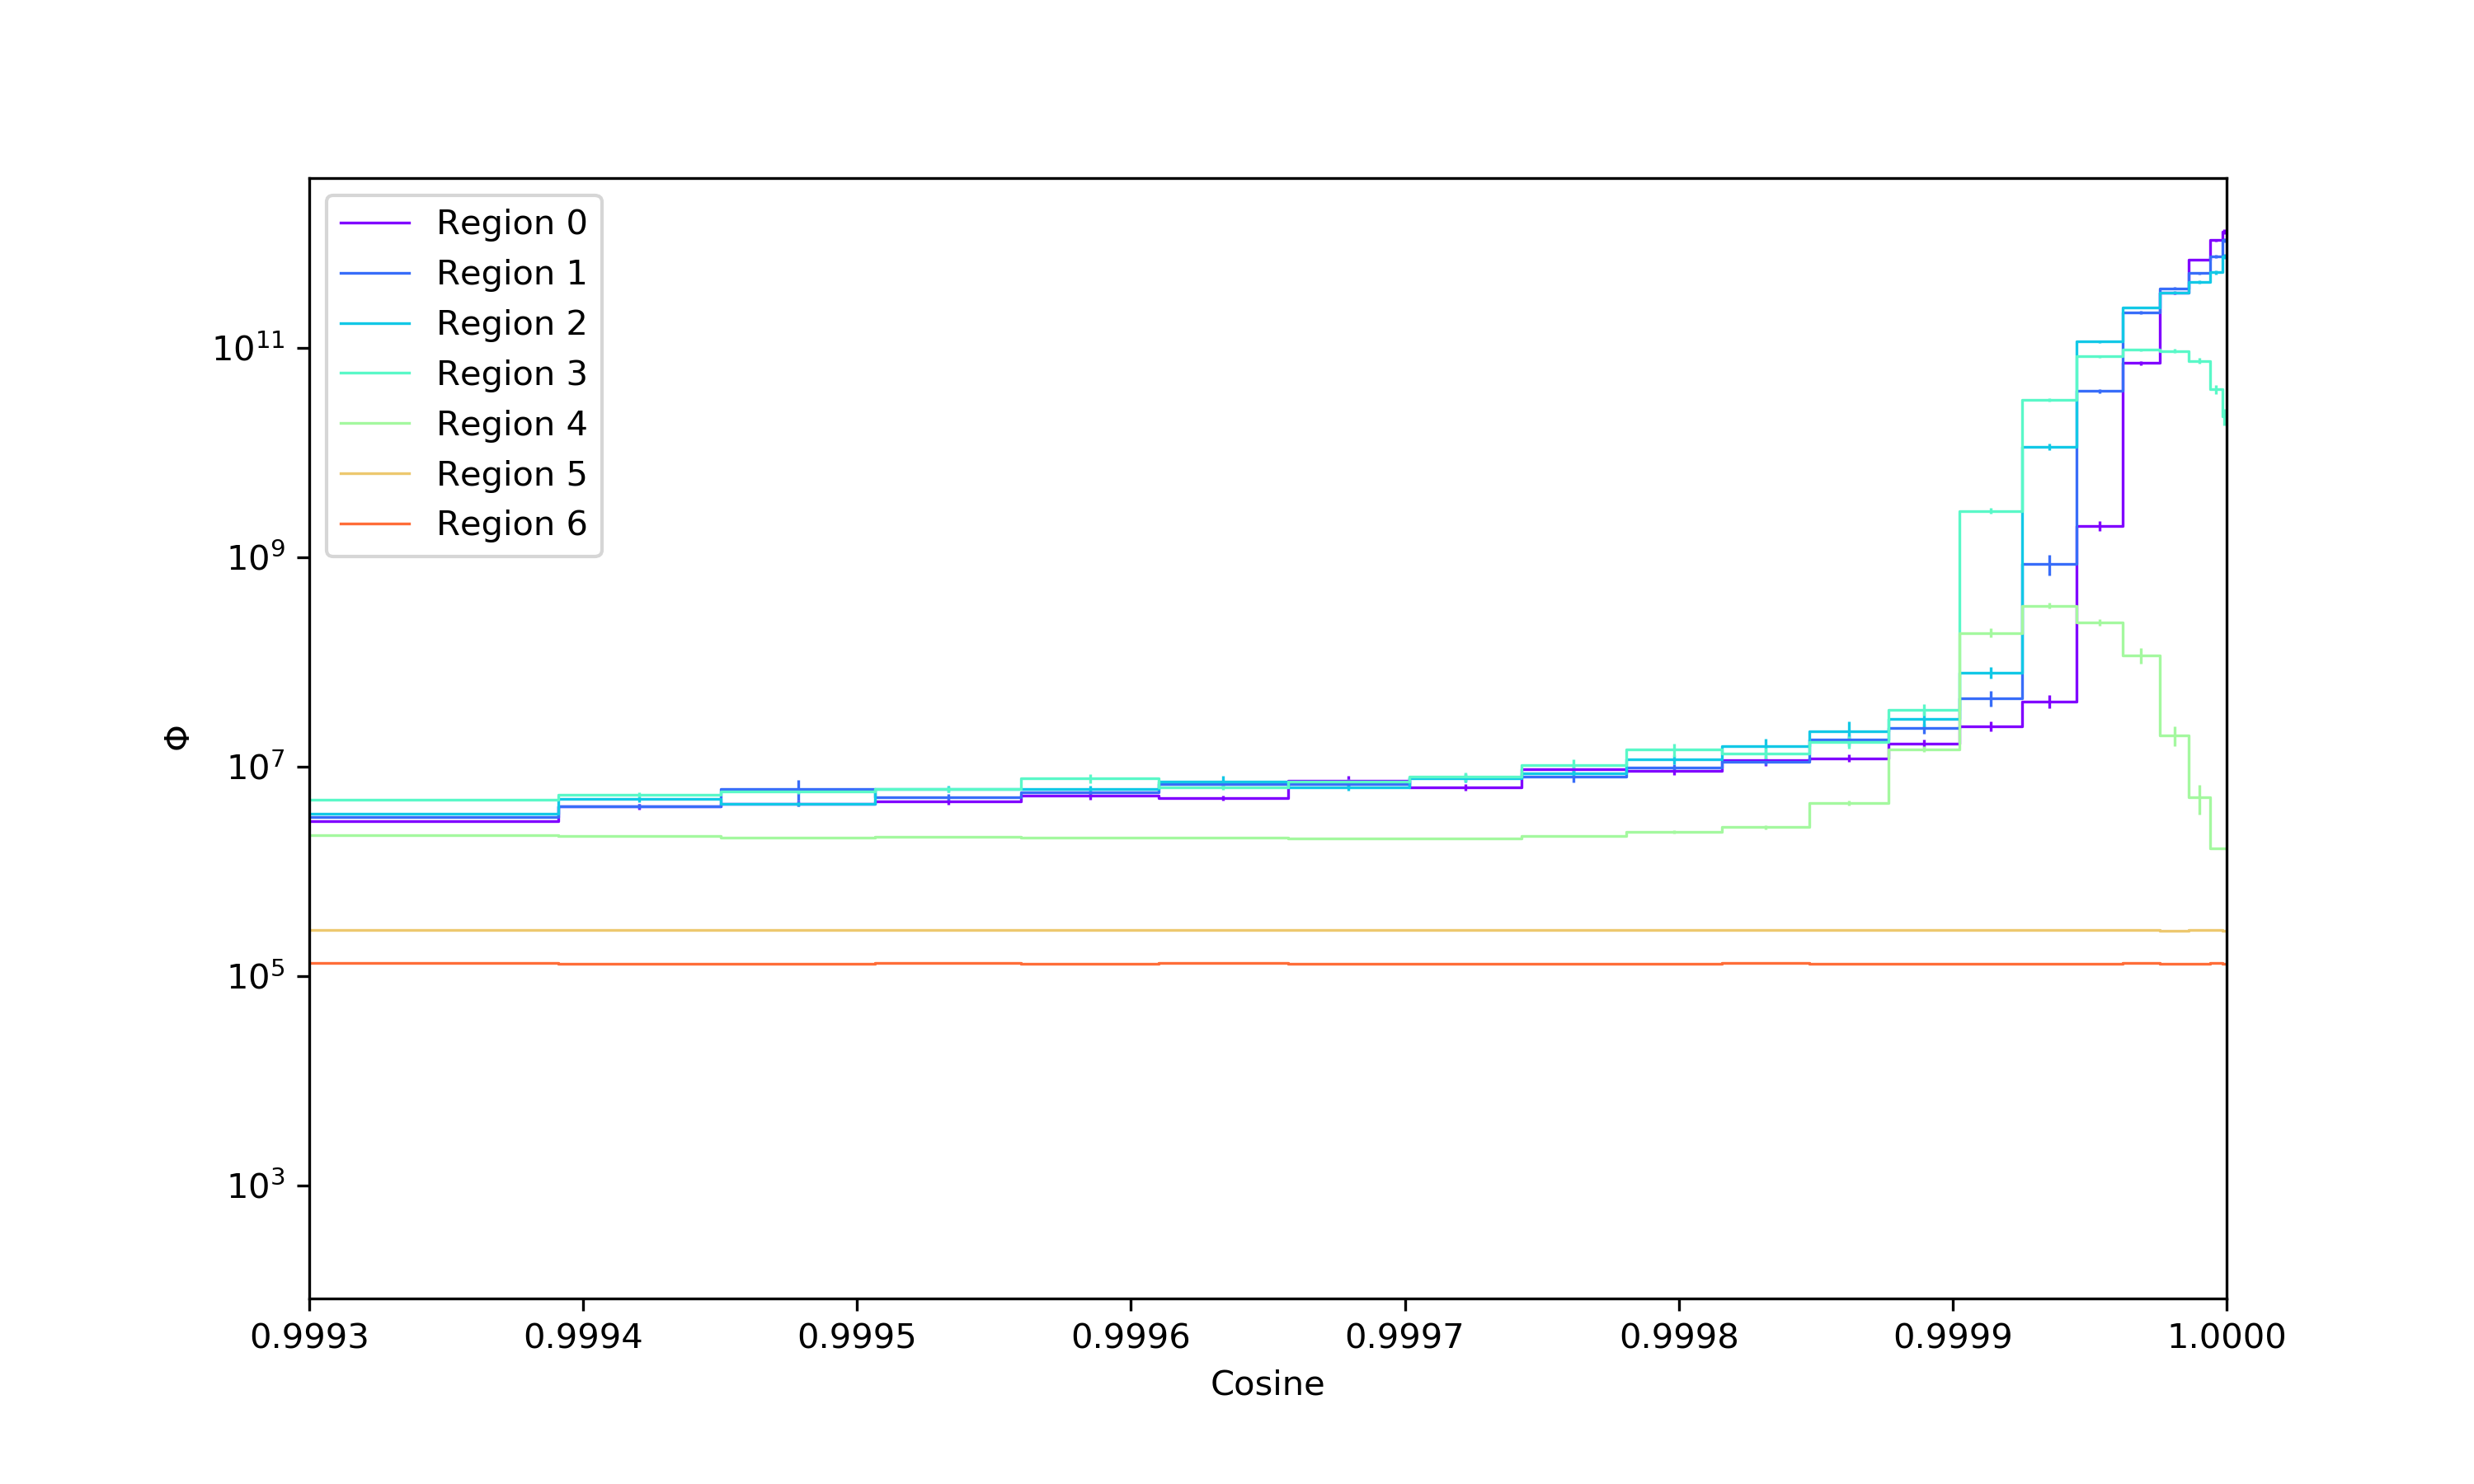
\includegraphics[height=4in]{tex/figures/flux_rad_cos_detail.png}
\caption[Detailed Regional Flux vs. Angle]{A detailed view of the angular flux broken into tally regions.}
\label{fig:flux_rad_cos_detail}
\end{figure}

% data shown in figure is a detailed view of the plot on the previous page
% this shows in greater detail the specifics of the forward peaking that happends in the angular flux
% regions 0-2 all have the highest bin being the most forward, however the distribution broadens as you move outward
% this trend is even true in the aluminum
% in the BP in region 4, the peak lies slightly off center, likely related to scattering behavior that allowed neutrons to get to that tally
% in this view, regions 5 and 6 appear isotropic, likely because a neutron to encounter one of those tally planes would have scattered several times

\clearpage

% the flux as a function of tally region
\begin{figure}[htb]
\centering
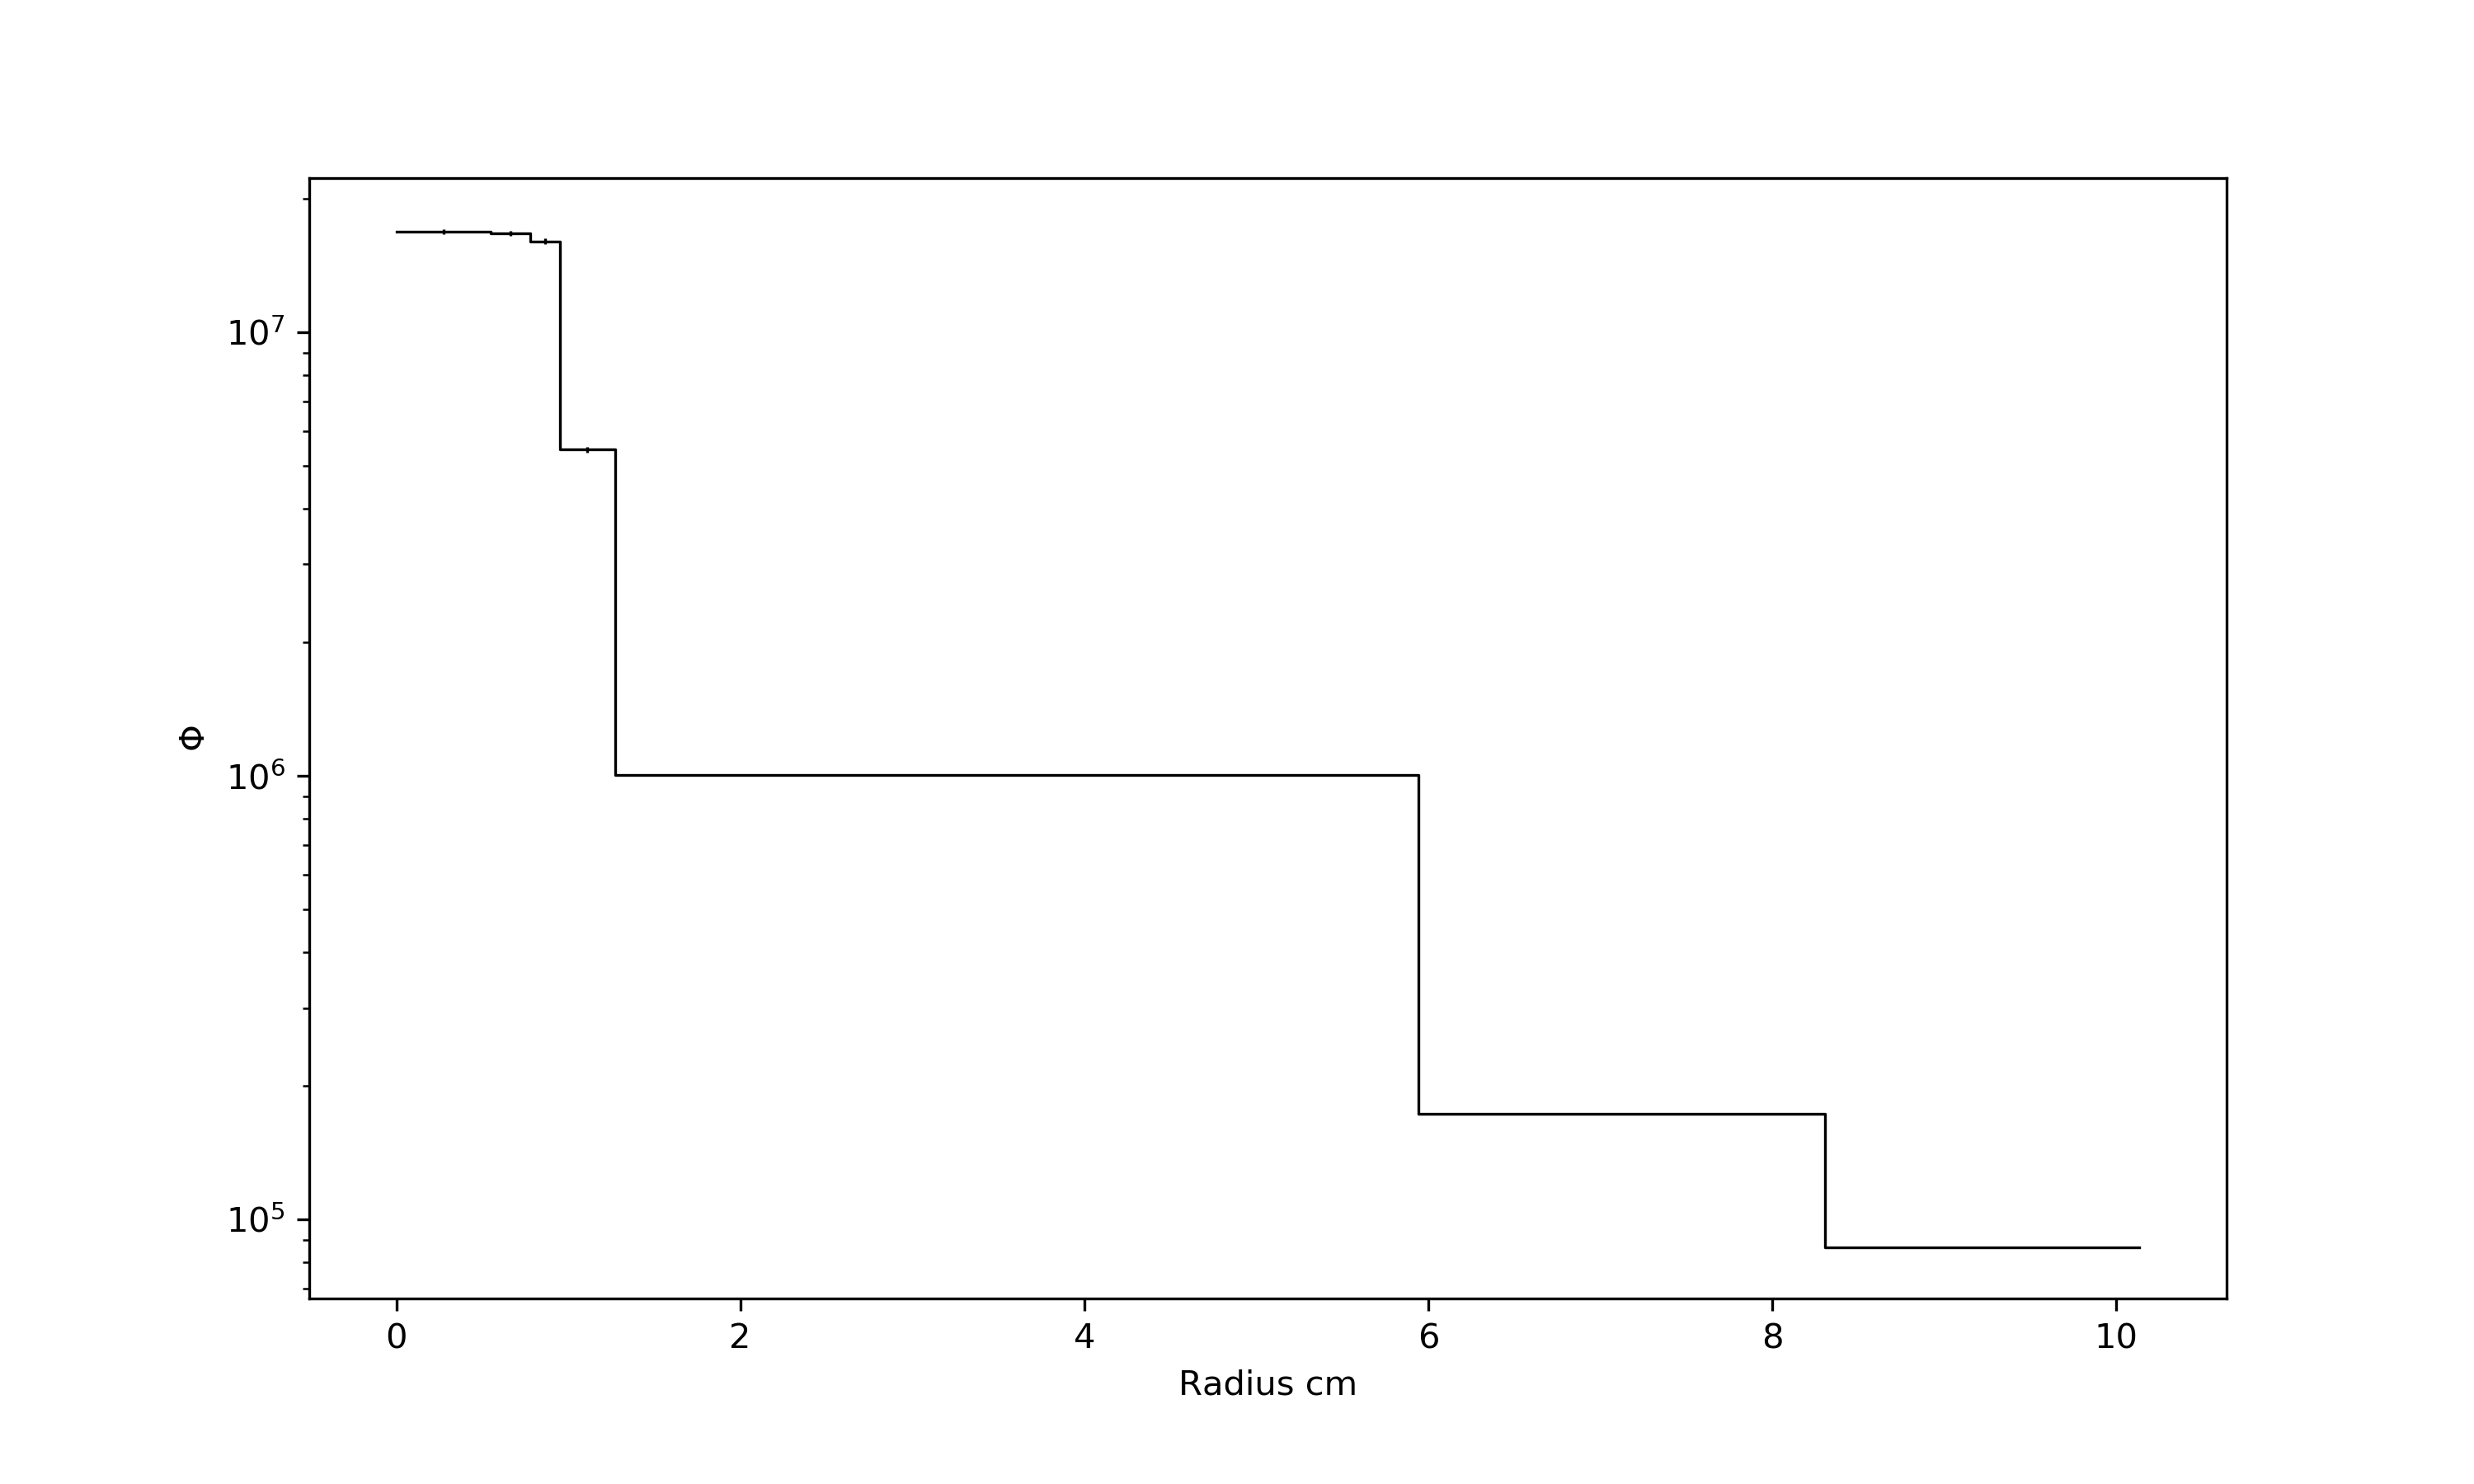
\includegraphics[height=4in]{tex/figures/flux_rad.png}
\caption[Regional Flux]{The NEBP flux as a function of tally region.}
\label{fig:flux_rad}
\end{figure}

% here, finally, we can see a direct comparison of the fluxes within each region of the tally
% there is very little difference between the tallies within the beam port
% then, from each region in the collimator, we see a tapering that leads to a two order of magnitude difference in the flux from the innermost to outermost region


\clearpage
